\documentclass[aspectratio=169, french]{beamer}
\usepackage{fontspec}
\usepackage[french]{babel}
\usefonttheme[onlymath]{serif}
\usepackage{amsmath,amssymb,amsthm}
\usepackage{arydshln,mathtools}
\usepackage{bm}
\usepackage{color}
\definecolor{theme}{RGB}{0,73,114}
\usepackage{multicol}
%\usepackage[caption=false]{subfig}
\usepackage{subcaption}

\usepackage{comment}

\usepackage{graphicx}
\usepackage{diffcoeff}
\usepackage{dsfont}
\usepackage{mathrsfs}
\usepackage[most]{tcolorbox}

\usepackage{xspace}
\usepackage{appendixnumberbeamer}


\usepackage{media9}
\usepackage[backend=bibtex, style=verbose]{biblatex}
\bibliography{biblioTrEquation}
%\renewcommand\bibfont{\scriptsize}

\addtobeamertemplate{footnote}{\vspace{-6pt}\advance\hsize-0.5cm}{\vspace{6pt}}
\makeatletter
% Alternative A: footnote rule
\renewcommand*{\footnoterule}{\kern -3pt \hrule \@width 2in \kern 8.6pt}
% Alternative B: no footnote rule
% \renewcommand*{\footnoterule}{\kern 6pt}
\makeatother

\graphicspath{{./images/}}



% Math macros
\DeclareMathOperator*{\grad}{grad}
\DeclareMathOperator*{\Grad}{Grad}
\DeclareMathOperator*{\Div}{Div}
\renewcommand{\div}{\operatorname{div}}
\DeclareMathOperator*{\Hess}{Hess}
\DeclareMathOperator*{\curl}{curl}
\DeclareMathOperator{\Tr}{Tr}
\DeclareMathOperator{\Dom}{Dom}
\DeclareMathOperator*{\esssup}{ess\,sup}

\newcommand{\bbR}{\mathbb{R}}
\newcommand{\bbF}{\mathbb{F}}
\newcommand{\bbA}{\mathbb{A}}
\newcommand{\bbB}{\mathbb{B}}
\newcommand{\bbS}{\mathbb{S}}

\newcommand*{\norm}[1]{\ensuremath{\left\|#1\right\|}}
\newcommand{\where}{\qquad \text{where} \qquad}
\newcommand{\inner}[3][]{\ensuremath{\left\langle #2, \, #3 \right\rangle_{#1}}}
\newcommand{\bilprod}[2]{\left\langle \left\langle \, #1, #2 \, \right\rangle \right\rangle}
\newcommand{\pder}[2]{\ensuremath{\partial_{#2} #1}}
\newcommand{\dder}[2]{\ensuremath{\delta_{#2} #1}}
\newcommand{\secref}[1]{\S\ref{#1}}
\newcommand{\energy}[1]{\frac{1}{2} \int_{\Omega} \left\{ #1 \right\} \d\Omega}
\newcommand{\crmat}[1]{\ensuremath{\left[#1\right]_\times}}
\newcommand{\fenics}{\textsc{FEniCS}\xspace}
\newcommand{\firedrake}{\textsc{Firedrake}\xspace}

\DeclareMathOperator*{\argmax}{arg\,max}
\DeclareMathOperator*{\argmin}{arg\,min}

\newtheorem{proposition}{Proposition}
\newtheorem{remark}{Remark}
\newtheorem{hypothesis}{Hypothesis}
\newtheorem{assumption}{Assumption}
\newtheorem{conjecture}{Conjecture}


\def\onedot{$\mathsurround0pt\ldotp$}
\def\cddot{% two dots stacked vertically
	\mathbin{\vcenter{\baselineskip.67ex
			\hbox{\onedot}\hbox{\onedot}}%
}}



\makeatletter \renewcommand\d[1]{\ensuremath{%
		\;\mathrm{d}#1\@ifnextchar\d{\!}{}}}
\makeatother


\graphicspath{{./imagesEqTr/}}


\begin{document}
	
	
\begin{frame}[plain]
	
	%%%%%%%% Title slide details %%%%%%%%%%%%%%


% Background Image
\newcommand{\myBackground}
{
    
\includegraphics[height=1.02\paperheight,page=9]{beamerthemeutresources}
}

% Title
\newcommand{\myTitle}
{
Méthodes des différences finies
}

% Subtitle
\newcommand{\mySubTitle}
{
EDP de transport 1D
}

% Author
\newcommand{\myAuthor}   
{
    Andrea Brugnoli
}

% Affiliation
\newcommand{\myAffiliate}
{
  
}

% Presentation Date
\newcommand{\myDate}   
{
    11 Avril 2022
}

% Logo
\newcommand{\myLogo}   
{
    
\includegraphics[width=3cm]{Logo.png}
}
%%%%%%%%%%%%%%%%%%%%%%%%%%%%%%%%%%%%


%%%%%%%%%% Title slide code %%%%%%%%%%%
\begin{tikzpicture}[remember picture,overlay]

% Background color

\fill[white] (current page.south west) rectangle (current page.north east);
% Background image
\node[above right,inner sep=0pt] at (current page.south west)
    {
        \myBackground
    };
    
% Title & Subtitle
\node
[
    above=0.5cm,
    align=center,
    draw=black!50,
    % rounded corners,
    double,
    double distance=0.1cm,
    double=blue!10,
    fill=theme!10,
    inner xsep=15pt,
    inner ysep=10pt, 
    minimum width=0.8\textwidth,
    text width=0.8\textwidth
] (title) at (current page.center)
{
    \LARGE \myTitle  \\[5pt]
    \small \mySubTitle
};

% Author 
\node[ below=0.5cm] (author) at (title.south){\myAuthor};

% Author 
\node[ below=0.25cm ](affiliate) at (author.south){\small \myAffiliate};

% Date
\node[below=0.25] (date) at (affiliate.south){\large \myDate};

% Logo
\node
[
    below =0.25cm
] at (date.south)
{
    \myLogo
};

\end{tikzpicture}
	
\end{frame}
	
	
\begin{frame}{Aperçu}
	
	\tableofcontents
	
\end{frame}

\section{Équation du transport 1D : le cas continu}

\begin{frame}{Équation du transport 1D}
	\begin{tcolorbox}[title = L'EDP la plus simple, coltitle=white]
		L'évolution d'un champ scalaire $u(x, t)$ transporté par un fluide satisfait 
		\begin{equation*}
			\diffp{u}{t} + \diffp{q}{x} = 0, \qquad x \in [0, L], \quad t \in  (0, T]. 
		\end{equation*}
	\end{tcolorbox}

\begin{tcolorbox}
	Pour le flux $q(u, x, t)$ on considère une vitesse constante pour le fluide
	\begin{equation*}
		q(u, x, t) = c \ u(x, t), \qquad c>0.
	\end{equation*}
	Le problème est bien posé lorsque on spécifie 
	\begin{align*}
		u(x, 0) &= g(x), \qquad \text{Donnée initiale}, \\
		u(0, t) &= f(t), \qquad \text{Condition au bord}.
	\end{align*}
\end{tcolorbox}

\end{frame}

\begin{frame}{Solution Analytique}
	Si $f, \; g$ sont régulières, i.e. $C^{1}$, et $f(0) = g(0), \; f'(0) = -c g'(0)$
alors  $u \in C^1([0, T]\times[0, L])$ 
\begin{equation*}
	u(x, t) = \begin{cases}
	g(x - ct), \quad &x\ge ct\\
	f(t-x/c), \quad &x\le ct,
	\end{cases}
	\qquad\text{i.e. $u$ constant sur $\gamma$ telle que $\dot{\gamma} = (c ,1)$.}
\end{equation*}

\begin{columns}
	\begin{column}{.4\textwidth}
	Exemple : $c=2, \quad L=20, \quad T = 10$
	\begin{align*}
		g(x) &= \exp(-x^2/4), \\
		f(t) &= \only<1>{1,}  \only<2>{\exp(-t^2),}  \only<3>{\cos^2(t),}
 	\end{align*}
	\end{column}
	\begin{column}{.6\textwidth}
		\begin{figure}
			\centering
			\only<1>{\includegraphics[height=.65\textheight]{u_sol_f1.eps}}
			\only<2>{\includegraphics[height=.65\textheight]{u_sol_f2.eps}}			
			\only<3>{\includegraphics[height=.65\textheight]{u_sol_f3.eps}}
		\end{figure}
	\end{column}
\end{columns}	

\end{frame}

\section{Discrétisation par différence finies}

\begin{frame}{Discrétisation du domaine : le maillage}
On considère un maillage rectangulaire uniforme $(t_j, x_m)$ : \\
cela signifie que $\Delta x = x_{i+1}- x_i $ et $\Delta t = t_{n+1}- t_n$ sont constants. \\
  \vspace{.5cm}
La champs scalaire discret est noté par $u_{i, n} \approx u(x_i, t_n)$ et représente une approximation de la solution exact.


\begin{figure}
\includegraphics[height=.6\textheight]{mesh.eps}
\caption*{Exemple de maillage rectangulaire uniforme : $\Delta x = L/10, \quad; \Delta t=T/10$.}
\end{figure}
	
\end{frame}

\begin{frame}{Approximation des dérivées}
	\begin{block}{Premier essai : schema d'Euler explicite}
		On considère l'approximation au premier ordre
		\begin{equation*}
			\diffp{u}{t}(x_i, t_j) \approx \frac{u_{i, n+1} - u_{i, n}}{\Delta t} + O(\Delta t), \qquad \diffp{u}{x}(x_i, t_j) \approx \frac{u_{i+1, n} - u_{i, n}}{\Delta x} + O(\Delta x) 
		\end{equation*}
	\end{block}
\end{frame}




\begin{frame}{Bibliographie}
	%\bibliographystyle{unsrt}
	\nocite{*}
	\printbibliography
\end{frame}
	
	
\end{document}